\documentclass[11pt,dvipdfmx]{ujarticle}
\usepackage{eee,scalefnt,graphicx}

\bibliography{3rd_hysteresis}
\begin{document}

\begin{jikkenTitle}
 \gakunen{3} 
 \numTitle{4}{変圧器を用いた磁性体の磁気特性観測} 
 \subTitle{(Observation of magnetic material using transformer)} 
 \jikkenbi{令和04年07月14日(木)} 
 \jikkenbiII{令和04年07月21日(木)}
 \kyoudou{3301 青木 柊人 3305 市川 潤} 
 \kyoudouII{3313 亀田 知典} 
 \yoteibi{07/21}
 \yoteibiII{07/28}
 \yoteibiIII{08/04}
 \hanNumberName{1}{3309}{大山 主朗}
\end{jikkenTitle}

\section{目的}
本実験では
\begin{itemize}
	\item トランス鉄心に使用される強磁性体のB-H特性測定を通し磁気回路と磁性材料について理解する.
	\item 変圧器鉄心の交流化特性を測定し,測定原理と鉄心のヒステリシス損算出法を理解する.
	\item 変圧器における励磁電流,電力,位相差の変化を観測する.
\end{itemize}
ことを目的とする.

\clearpage

\section{原理}
\subsection{磁気回路(Magnetic circuit)}
\wfig{hys:jikikairo}に示すように断面積$S\,[\mathrm{m}^2]$,平均磁路長$L\,[\mathrm{m}]$の鉄心に巻数$N_1\,[\mathrm{Turn}]$のコイルを巻き,これに$I\,[\mathrm{A}]$の電流を流すと,起磁力$N_1\cdot I\,[\mathrm{A}\cdot\mathrm{Turn}]$を生じる.
この起磁力により
\begin{equation}
	\phi = \frac{N_1\cdot I}{R_m}
\end{equation}
の磁束$\phi\,[\mathrm{Wb}]$を生じる.ここで$R_m$は以下に示す磁気抵抗である.
\begin{equation}
	R_m= \frac{L}{\mu_0 \mu_s S}
\end{equation}
ただし,$\mu_0 = 4\pi\times 10^{-7}\,\mathrm{F/m}$ は真空の透磁率であり,$\mu_s$は鉄心の比透磁率である.
ここで,磁路1\,mあたりの起磁力を磁化力$H\,[\mathrm{A/m}]$という. 磁化力$H$は
\begin{equation}
	H=\frac{N_1\cdot I}{L}
\end{equation}
である.また磁路断面積 1\,m$^2$あたりの磁束を,磁束密度$B\,[\mathrm{Wb/m}^2]$という.
\begin{equation}
	B=\frac{\phi}{S}
	\label{eq:hys:BphiS}
\end{equation}
ここで,$S\,[\mathrm{m}^2]$は磁路断面積を示す.
\begin{figure}[htbp]
	\centering
	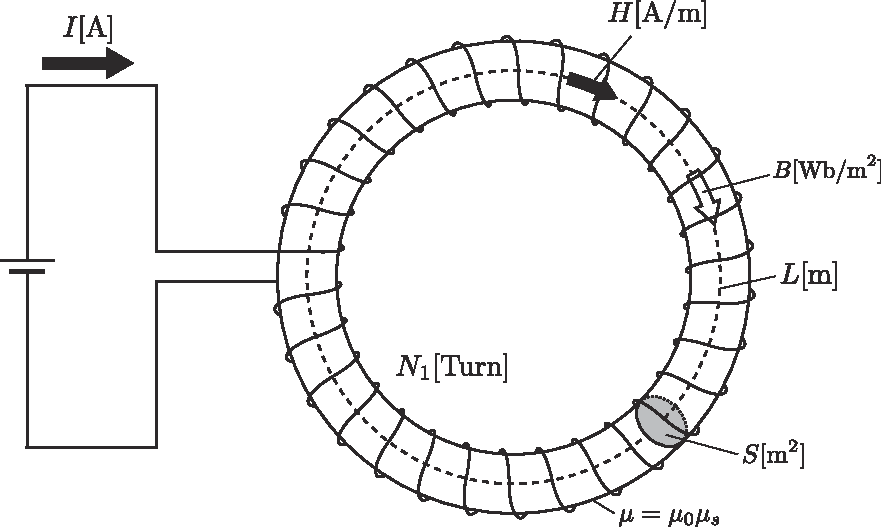
\includegraphics[width=70mm]{fig/magnetism_circuit.pdf}
	\caption{磁気回路}
	\label{fig:hys:jikikairo}
\end{figure}

鉄心の磁化力$H$と磁束密度$B$との関係を示す曲線をB-H曲線といい,一般に\wfig{hys:bhcurve}(a)のような飽和特性になる.
また磁化力$H$を正負の方向に増減すると,\wfig{hys:bhcurve}(b)の様なヒステリシス曲線(Hysteresis curve)になる.
\begin{figure}[htbp]
	\centering
	\begin{tabular}{cc}
		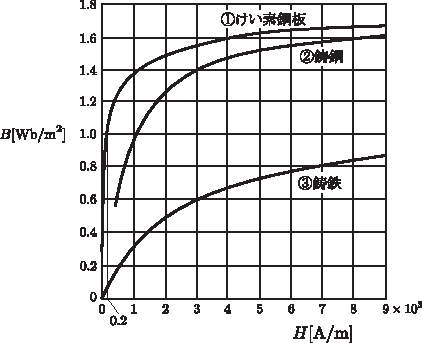
\includegraphics[width=70mm]{fig/bhcurve.pdf} &
		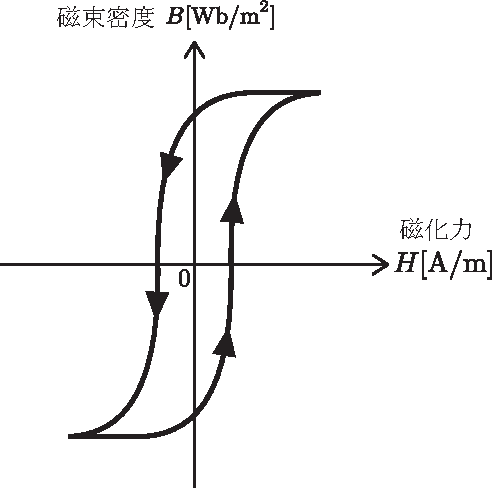
\includegraphics[width=70mm]{fig/hysteresis.pdf} \\
		(a) B-H 曲線 & (b) ヒステリシス曲線
	\end{tabular}
	\caption{B-H曲線とヒステリシス曲線}
	\label{fig:hys:bhcurve}
\end{figure}

\subsection{交流磁化特性}
\label{zika}
\wfig{hys:transformer}の変圧器のように,鉄心に巻かれた巻数$N_1$のコイルに交流電圧$V_1$を加えると,鉄心中に交番磁束$\dot{\phi}$を作るための電流(励磁電流)$i_0$が流れる.このとき磁束密度$B$と磁化力$H$との間にはヒステリシス特性があるため,励磁電流は\wfig{hys:hizumi}のようにひずみを生ずる.この現象を逆に利用して,励磁電流$i_0$と交番磁束$\dot{\phi}$の波形をなんらかの方法で取り出し,オシロスコープのX軸に励磁電流$i_0$の波形,Y軸に交番磁束$\dot{\phi}$の波形を入力すれば,オシロスコープの画面に鉄心のヒステリシス特性(B-H曲線)が描かれる.
\begin{figure}[htbp]
	\centering
	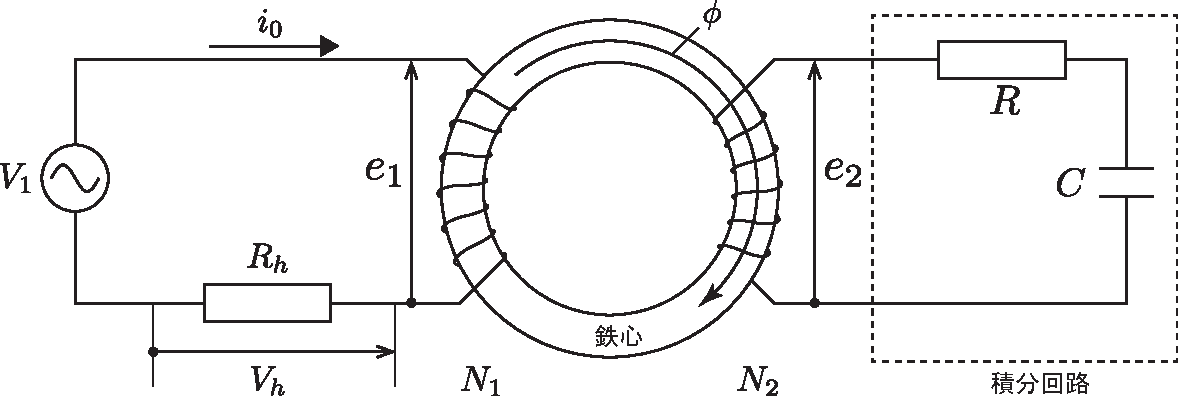
\includegraphics[width=140mm]{fig/transformer.pdf}
	\caption{変圧器の交流磁化特性測定回路}
	\label{fig:hys:transformer}
\end{figure}

励磁電流$i_0$の波形を直接取り出すのは難しいので,\wfig{hys:transformer}において励磁電流$i_0$が抵抗$R_h$を流れるときの電圧変化,すなわち
\begin{equation}
	V_h = i_0R_h
\end{equation}
として取り出す.また,交番磁束$\dot{\phi}$は次の様にして取り出す.

\wfig{hys:transformer}において二次巻線$N_2$と鎖交する磁束の時間に対する変化が二次誘起電圧$e_2$として現れるため
\begin{equation}
	e_2 = -N_2\frac{d \phi}{dt}
	\label{eq:hys:e2}
\end{equation}
となり,\weq{hys:e2}を変形すると
\begin{equation}
	d \phi = \frac{1}{N_2}\times e_2\times dt
	\label{eq:hys:dphi}
\end{equation}
となるから,交番磁束$\phi$は\weq{hys:dphi}を積分すれば求まることとなる.すなわち,二次巻線に発生する電圧$e_2$を時間で積分すればよい.そこで二次側にCR積分回路を接続しコンデンサCの両端から$e_2$を積分した,交番磁束に比例した電圧をとりだす.

\begin{figure}[h]
  \begin{minipage}[c]{0.5\hsize}
    \centering
    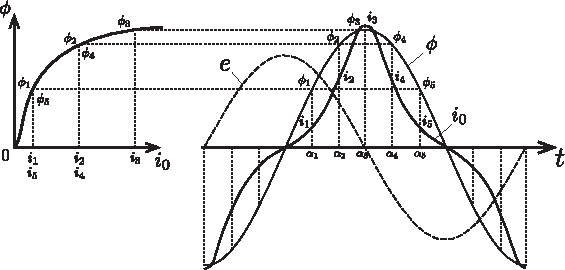
\includegraphics[scale=1.2]{fig/hizumi_a.pdf} 
    \caption{ヒステリシス現象のない場合}
  \end{minipage}\\
  \begin{minipage}[c]{0.5\hsize}
    \centering
    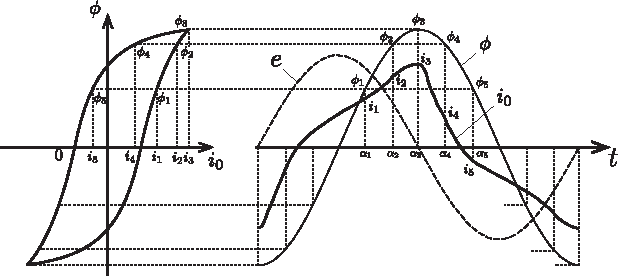
\includegraphics[scale=1.2]{fig/hizumi_b.pdf}
    \caption{ヒステリシス現象のある場合}
  \end{minipage}
  \centering
  \caption{ヒステリシス現象}
   \label{fig:hys:hizumi}
\end{figure}

\subsection{磁区}
\subsection{理想変圧器}
\subsection{実際の変圧器}
\subsection{磁気飽和現象}\label{hohwa}
\subsection{抵抗損と漂遊負荷損\cite{1130282271832577152}}
ブリッジ法などで測定した巻線の抵抗(直線抵抗)を$r_{d}$とし,巻線に流れる交流電流を$I$とすると,抵抗損は$I^{2}r_{d}$である.しかし,実際の損失はこの値より大きくなる.その理由は次の2つである.
\begin{enumerate}[(1)]
	\item \textbf{導体内のうず電流損}\\
	電流による漏れ磁束が導体自身の断面に鎖交するため,導体内にうず電流が発生し,電流密度が不均一になり,導体断面積が減少したのと同じ結果となり抵抗が増加する.またその増加分は$5 \sim 20\,\%$である.また,うず電流は抵抗に反比例するため,巻線の断面積が大きい場合はうず電流を低減することができる\cite{11302822718325772}\cite{1130282270467697152}.
	\item \textbf{構造材料内の損失}\\
	漏れ磁束の一部は,タンクの側板,締め付けボルトなどを通るため,それらの部分にうず電流損失やヒステリシス損失が生じる.以上の2つを合わせて漂遊負荷損といい,抵抗損の$5 \sim 20\,\%$になる.
	抵抗損と漂遊負荷損の和が負荷損であるが,その値はほとんど電流の2乗に比例する.すなわち,二次負荷電流を$I_{2}$とすれば負荷損$W_{l}$は
	\begin{equation}
		W_{l}=I_{2}^{2}r
	\end{equation}
	で表される.
\end{enumerate}

\subsection{積分回路}
\subsection{電流密度}

\newpage
\section{方法}
\subsection{使用器具}
今回の実験で使用した器具を\wtab{kigu}に示す.\\
なお,実験指導書ではソフトが``NI LabVIEW2015(32ビット)''と記載されていたが,使用したPCにインストールされていたものは``NI LabVIEW2019SPI(32ビット)''であった.

\begin{table}[hbtp]
  \centering
  \caption{実験装置}
  \label{tab:kigu}
  \scalebox{0.75}{
  \begin{tabular}{cccccc}
    \hline
    機器名&製造元&型番&シリアル番号&数量\,個\\
    \hline
    PC&iiyama&NK50SZ&NKNK50SZ0000K00088&1\\
    組み込みデバイス&NATIONAL INSTRUMENTS&myRIO-1900&308778E&1\\
    ブレッドボードアクセサリ&DEGILENT&MXP Breadboard for NI myRIO&D535760&1\\
    ソフトウェア&NATIONAL INSTRUMENTS&LabVIEW&LabVIEW2019 19.0.H3(32-bit)&1\\
    \hline
  \end{tabular}
  }
\end{table}

\subsection{実験手順}
プログラムの実行が速く,目視による確認が難しい場合,``ハイライトモード''を有効にすると実行過程がゆっくり表示されるようになる.
また以下では,基本的なLabVIEWの操作方法については述べない.
\subsection{実習2-1}
\subsubsection{導通確認}
\begin{enumerate}[a)]
	\item MXPブレッドボードアクセサリとジャンパーワイヤーを使って\wfig{2.12}のように回路を構築.その後,アクセサリボードをmyRIOのAポートに接続.
	\item ブロックダイアグラムで,``Analog Input''(Channel欄には,``A/AI 0(pin3)''を選択)を配置し,同右コネクタ(A/AI 0 pin3)に,``表示器''を作成.
	\item 上の計測プログラムを実行.
	\item \wfig{2.12}において``接続先を変更する''と記載されている端子をGND, 3.3\,\rm{V}, 5\,\rm{V}それぞれに接続し,値が正しく変化することを確認した.
\end{enumerate}
\begin{figure}
\centering
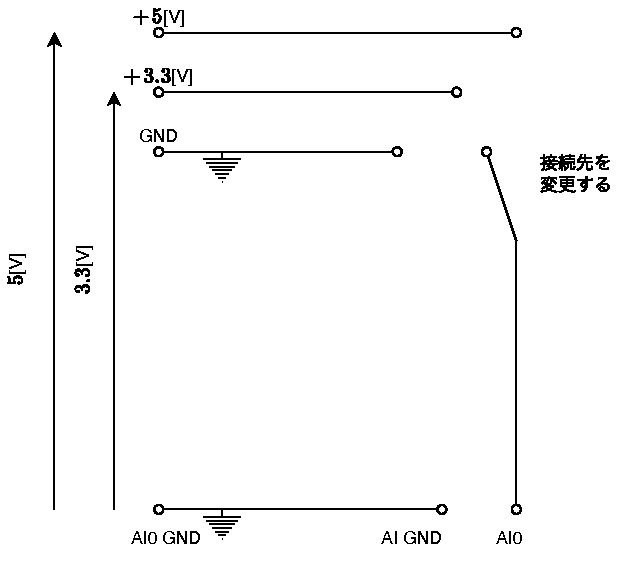
\includegraphics[scale=0.7]{/Users/ohyamasan/Downloads/TMCIT-Report/EE_Measurement/fig/100-volt.pdf}
\caption{定電圧計測回路}
\label{fig:2.12}
\end{figure}

\subsubsection{``For ループ''}
\begin{enumerate}[a)]
	\item 上で作成した``Analog Input''ブロックと表示器とを``Forループ''で囲むように配置し,``i''に表示器を作成.
	\item ``For ループ''のコネクタ``N''に定数を作成し5を代入.
	\item 上記プログラムを実行し正しく動作していることを確認した.
	\item ``Analog Input''の右コネクタ(A/AI 0 pin3)と``For ループ''の右端枠に接続し,コネクタに表示器を作成.(名前が``配列''に変更される)
	\item 作成したプログラムを実行し.``配列''(フロントパネル上の)に表示器(A/AI0)に表示された値が表示されることを確認した.
\end{enumerate}

\subsubsection{``配列連結追加''}
\begin{enumerate}[a)]
	\item 上の``For ループ''プログラムに``配列連結追加''ブロックを配置し,同左コネクタをカウンタ変数``i''に接続.
	\item ``配列連結追加''の左コネクタに``入力を追加''を選択し,数値入力用の左コネクタが2つになることを確認した.
	\item ``配列連結追加''ブロックの左コネクタを``Analog Input''の右コネクタ(A/AI 0 pin3)に接続.
	\item ``配列連結追加''の右コネクタを``For ループ''の右端枠に接続し,コネクタに表示器を作成.(名前が``配列2''に変更される)
	\item フロントパネルの“配列2”を選択し,5段以上表示されるように変更.
	\item 作成したプログラムを実行し,``配列2''に``i''の値と電圧値が2列で表示されることを確認した.
\end{enumerate}

\subsubsection{``配列からスプレッドシート文字列に変換''}
\begin{enumerate}[a)]
	\item ブロックダイアグラムに``配列からスプレッドシート文字列に変換''ブロックを配置.左上コネクタ(形式文字列)は空欄のまま.
	\item ブロックの左下コネクタ(配列)を``For ループ''枠右コネクタ``配列2''と接続.
	\item ブロックの被疑コネクタ(スプレッドシート文字列)に表示器を作成.(名前が``スプレッドシート文字列''に変更される)
	\item 作成したプログラムを実行し,``配列''に``i''と電圧値が2列で表示されることを確認した.
	\item フロントパネルの``スプレッドシート文字列''をトリプルクリックすると全て選択でき,Excelにペースト可能であることを確認した.
\end{enumerate}

\subsection{実習2-1 課題実験}
\begin{enumerate}[a)]
\item 100回のデータ計測をするようにプログラムを変更.
\item GND, 3.3\,\rm{V}, 5\,\rm{V}の出力電圧を100回分計測し,Excelを用いて平均値と標準偏差を求めた.
\end{enumerate}

\subsection{実習2-2}
\subsubsection{定電圧計測}
\begin{enumerate}[a)]
	\item ブロックダイアグラムに``Analog Input''を配置.Cnfiguration 画面のChannel 欄には,電圧入力ピンとして``A/AI0 (pin3)''を選択.
	\item``Analog Input''の右コネクタ(A/AI0 pin3)に``表示器''を作成.``Analog Output''を追加.
	\item Configuration 画面のChannel 欄には,電圧出力ピンとして``A/AO 0 (pin2)''を選択.
	\item ``Analog Output''の左コネクタ(A/AO 0 pin2)に``制御器''を作成.
\end{enumerate}

\subsubsection{出力電圧値変化}
\begin{enumerate}[a)]
	\item ブレッドボードアクセサリを\wfig{5-volt}のように構築し,アクセサリボードをmyRIOのAポートに挿入.
	\item 上のプログラムを実行し,``数値表示器''(A/AI0 Pin3)に表示される値を確認した.
	\item ``制御器''(A/AO 0 pin2)に0\,\rm{V}から5\,\rm{V}の数値を入力する.複数回実行し,``数値表示器''(A/AI0 pin3)に表示される値を確認した.
	\item ``制御器''(A/AO 0 pin2)の数値をさらに変更し,上と同様に複数回実行し,値の変化を確認した.
\end{enumerate}

\begin{figure}[htb]
\centering
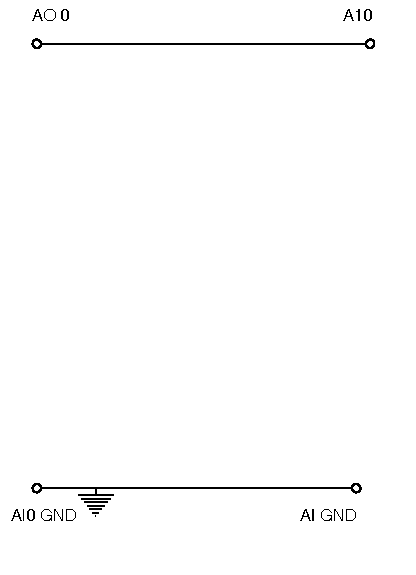
\includegraphics[scale=0.65]{/Users/ohyamasan/Downloads/TMCIT-Report/EE_Measurement/fig/5-volt.pdf}
\caption{変電圧計測回路}
\label{fig:5-volt}
\end{figure}

\subsubsection{出力電圧表示値と計測電圧値を配列・文字列で表示}
\begin{enumerate}[a)]
	\item 上記のプログラムの全てのプログラムを``For ループ''で囲むように配置.コネクタ``N''に定数を作成し,5を代入.
	\item ``Analog Output''の左コネクタ(A/AO 0 pin2)をカウンタ変数``i''に接続.(制御器``AO0''との接続は予め解除しておく)
	\item ``配列連結追加''ブロックを追加し,その出力コネクタから伸ばしたワイヤーを``For ループ枠''に繋げ,表示器を新規作成.
	\item 作成したプログラムを実行し,``配列''に表示される電圧値を予想される値と比較した.
	\item ブロックダイアグラムに``遅延時間''を追加し,制御器を追加.``遅延時間''は0.05\,秒に設定.
	\item ``AnalogOutput''の``error out''と``遅延時間''の``エラー入力'',``遅延時間''の``エラー出力''と``AnalogOutput''の``error in''を接続.
	\item ``遅延時間''ブロックの追加による``配列''に表示される値の変化を確認した.
	\item 遅延時間を,0\,秒, 0.005\,秒, 0.050\,秒, 0.500\,秒に変え,それぞれの場合で入力値を変更し,表示値との比較を行った.(3.5.2のように2回目以降は入力値と出力値がほぼ一致した)
	\item 以降の手順は3.3.3および3.3.4を参照し,文字列を表示させる.
\end{enumerate}


\subsection{実習2-2 課題実験}
\begin{enumerate}[a)]
	\item 0\,\rm{V}から5\,\rm{V}まで0.5\,\rm{V}刻みで出力電圧を変え,出力電圧値を計測.
	\item ``Analog Output''に入力した値・``Analog Input''から取得した値をカウンタ変数``i'', ``Analog Output''表示値・``Analog Input''表示値を表示.
	\item ``出力電圧表示値''と``計測電圧表示値''との差を表示.
	\item 上で導出した差から二乗平均平方根誤差(Root Mean Squared Error, RMSE)をExcelを用いて求めた.
\end{enumerate}


\subsection{実習3}
\subsubsection{固定抵抗の電圧電流特性}
\begin{enumerate}[a)]
	\item \wfig{mesure-vl}のように回路を構築.
	\item V, $V_{U}$, $R_{0}$を用いて電圧,電流を計測し電圧-電流特性を計測する.なお測定対象素子は,1\,k\rm{$\Omega$}.$R_{0}$の抵抗値変化は,100\,\rm{$\Omega$},1\,k\rm{$\Omega$},10\,k\rm{$\Omega$},100\,k\rm{$\Omega$}である.
\end{enumerate}

\begin{figure}[h]
\centering
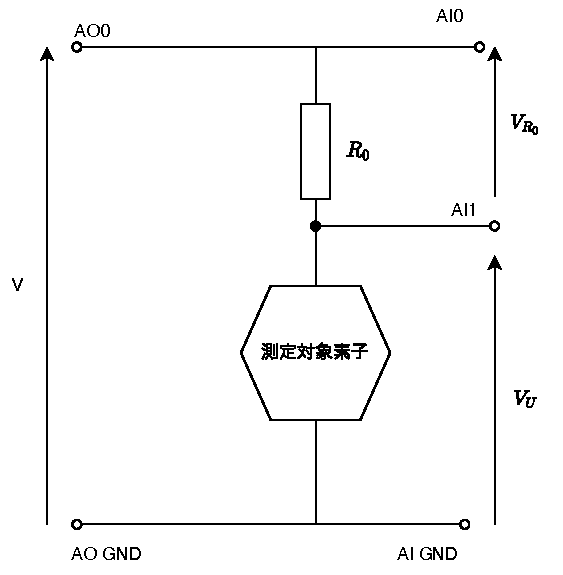
\includegraphics[scale=0.75]{/Users/ohyamasan/Downloads/TMCIT-Report/EE_Measurement/fig/mesure-vl.pdf}
\caption{電圧電流特性計測回路}
\label{fig:mesure-vl}
\end{figure}


\subsubsection{可変抵抗(ポテンショメータ)の電圧電流特性}
\begin{enumerate}[a)]
	\item \wfig{mesure-vl}において,測定素子を可変抵抗に変更.
	\item \wfig{poten}を参考にして,可変抵抗の端子間を1-2としてつまみ位置をA, B, C (くぼみが向いている向きがA, B, Cとなるように.すなわち,図ではAの状態である)にして,それぞれの電圧を計測した.なお,プログラムは上で作成したものをそのまま利用した.
	\item 可変抵抗の端子間を2-3, 3-1間でも同様に測定した.
	\item ただし,$R_{0}$は測定データを基に適切なものを選択した.
\end{enumerate}

\begin{figure}[h]
\centering
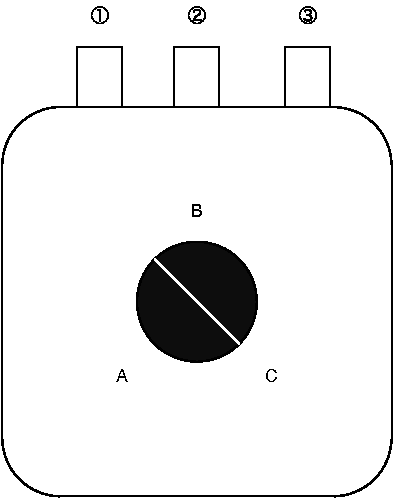
\includegraphics[scale=0.6]{/Users/ohyamasan/Downloads/TMCIT-Report/EE_Measurement/fig/potencial.pdf}
\caption{ポテンショメータ}
\label{fig:poten}
\end{figure}

\subsubsection{CdSセンサの電圧電流特性}
\begin{enumerate}[a)]
	\item \wfig{mesure-vl}の測定素子をCdSセンサ(\wfig{CdS})に変更.
	\item 自然状態とスマホのライトをセンサ部分に照射する場合のそれぞれで,上と同様に測定を行った.
	\item ただし,$R_{0}$は測定データを基に適切なものを選択した.
\end{enumerate}

\begin{figure}[h]
\centering
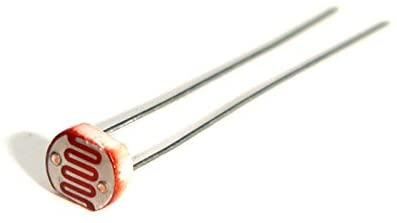
\includegraphics[scale=0.5]{/Users/ohyamasan/Downloads/TMCIT-Report/EE_Measurement/fig/31AbZ9saczL._AC_.jpg}
\caption{CdSセンサ\cite{cbs}}
\label{fig:CdS}
\end{figure}

\subsubsection{力センサの電圧電流特性}
\begin{enumerate}[a)]
	\item  \wfig{mesure-vl}の測定素子を力センサ(\wfig{power})に変更.
	\item 自然状態とセンサ部分(黒い枠で囲まれている円部分)を強く押し続けた状態のそれぞれで,上と同様に測定を行った.
	\item ただし,$R_{0}$は測定データを基に適切なものを選択した.
\end{enumerate}

\begin{figure}[h]
\centering
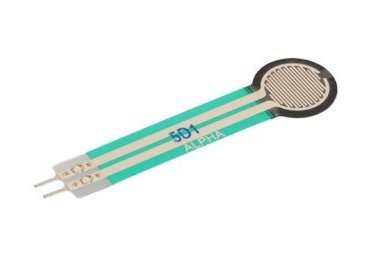
\includegraphics[scale=0.5]{/Users/ohyamasan/Downloads/TMCIT-Report/EE_Measurement/fig/31Gu87ucreL.jpg}
\caption{力センサ\cite{power}}
\label{fig:power}
\end{figure}

\subsubsection{発光ダイオードの電圧電流特性}
\begin{enumerate}[a)]
	\item \wfig{mesure-vl}の測定素子をLEDに変更.
	\item 測定するLEDは発光色4種類(赤,青,白,緑)で行った.
	\item ただし,$R_{0}$は測定データを基に適切なものを選択した.
\end{enumerate}
\clearpage

\section{結果}
\begin{itemize}
	\item 入力電圧-励磁電流-電力-電力の関係は\wtab{re1}のようになった.入力電圧上昇とともに電流,電力,位相の増加が確認できる.
	\begin{table}[h]
	\centering
	\caption{励磁電流特性}
	\label{tab:re1}
	\begin{tabular}{cccc}
	\hline
	入力電圧$V\,[\rm{V}]$& 電流$i_{0}\,[\rm{A}]$& 電力$P_{0}\,[\rm{W}]$& 位相\,[\rm{deg}]  \\ 
	\hline
	75  & 0.307    & 1.84     & 85.41643 \\
	80  & 0.337    & 2.10      & 85.53252 \\
	85  & 0.378    & 2.36     & 85.78774 \\
	90  & 0.429    & 2.64     & 86.07928 \\
	95  & 0.483    & 2.96     & 86.30133 \\
	100 & 0.552    & 3.34     & 86.53107 \\ \hline
	\end{tabular}
	\end{table}
\end{itemize}
\clearpage

\section{考察}
\subsection{課題考察}
\begin{enumerate}[1.]
	\item 変圧器の励磁電流について調べ,なぜ流れ,どのような役割をしているのかを考察せよ.\cite{1130282270091029760}
	
	実際の変圧器では,一次・二次巻線には抵抗があるため,負荷電流が流れると銅損が生じる.
	また,鉄心の透磁率は無限大ではないため,磁束$\dot{\phi}$をつくるために電流が必要となる.
	この電流を励磁電流(exciting current)という.
	これによって,鉄心中には鉄損が生じる.
	\item 励磁電流がひずみ波形になる理由を説明せよ.
	
	実際の変圧器では,一次巻線に交流電圧を加えると,鉄心の磁気飽和現象(参考:\ref{hohwa})やヒステリシス現象(参考:\ref{zika})が生じるため,励磁電流は非正弦波交流(ひずみ波形)となる\cite{1130282270091029760}.
	\item 磁性材料のヒステリシス損失について調査せよ.特に使用電圧が変化したとき及び使用電圧の周波数が変化したときについてそれぞれ説明せよ.\cite{11302822718577152}
	\label{hlos}
	
	ヒステリシス損は,鉄心内の磁束が方向及び大きさを変化することにより鉄心を構成する磁気分子が方向・配列を変え,分子相互間に摩擦損が生じることに起因するもの.
	また,ヒステリシスループの囲む面積に比例する.従って,周波数に比例し,さらに,最大磁束$\Phi_{m}$のとき磁束密度$B_{m}$がほぼ$1\,\rm{T}$以下では$B_{m}^{1.6}$に比例し,$1\,\rm{T}$以上では$B_{m}^{2}$に比例する.
	普通,$B_{m}=1 \sim 1.8\,\rm{T}$で使用されるため,鉄心の単位質量当たりのヒステリシス損$\omega_{h}$は以下で与えられる.
	\begin{equation}
		\omega_{h}=\sigma_{h}fB_{m}^{2}=k_{1}\frac{E^{2}}{f}\,[\rm{W/kg}]
		\label{eq:he}
	\end{equation}
	ここで,$\sigma_{h}$はヒステリシス損係数,$f\,[\rm{Hz}]$は周波数,$B_{m}\,[\rm{T}]$は最大磁束$\Phi_{m}$のときの鉄心磁束密度,$k_{1}$は比例定数,$E\,[\rm{V}]$は誘導起電力である.\\
	\weq{he}より使用電圧及び使用電圧の周波数が増加すると損失も増加することがわかる.
	\item 磁性材料のうず電流損について調査せよ.特に使用電圧が変化したとき及び使用電圧の周波数が変化したときについてそれぞれ説明せよ.\cite{11302822718577152}
	\label{uzu}
	
	うず電流損は,磁束の変化によって鉄心内に起電力を生じ,電流が流れる結果,抵抗損失が生じるもので,鋼板の厚さ,周波数及び磁束密度のそれぞれ2乗に比例する.
	これらより,単位重量当たりのうず電流損$\omega_{e}$は次式で与えられる.
	\begin{equation}
	\omega_{e}=\sigma_{e}t^{2}f^{2}B_{m}^{2}=k_{2}t^{2}E^{2}\,[\rm{W/kg}]
	\label{eq:uzue}
	\end{equation}
	ここで,$\sigma_{e}$はうず電流損係数,$t\,[\rm{mm}]$は積層鋼板1枚の厚さ,$k_{2}$は比例定数である.\\
	この\weq{uzue}より使用電圧及び使用電圧の周波数が増加すると損失も増加することがわかる.
	\item 電力計を使用して測定するときの損失とヒステリシス曲線から求めた損失について比較検討し考察せよ.\label{pi}
	
	ヒステリシス損は\ref{hlos}で述べたようにヒステリシスループ内の面積に比例し,\weq{w}を用いて算出することができる.
	なお,ヒステリシスループ内の面積はImageJを用いて算出した.
	また,保存したヒステリシスループの波形は$1\,\rm{DIV}=1\,\rm{cm}$となるように加工をしたため,$[\rm{cm^{2}}]=[\rm{DIV^{2}}]$である.
	\begin{align}
	W_{h}\,[\rm{W}]&=f\times A \times S\times L \times 換算\rm{X}軸測定条件\,[\rm{A/m\cdot 1/DIV}]\times 換算\rm{Y}軸測定条件\,[\rm{Wb/m^{2}\cdot 1/DIV}]\nonumber\\
	\label{eq:w}
	\end{align}
	ここで$A=3.84\times 10^{-4}\,\rm{m^{2}}$は鉄心断面積,$S\,[\rm{cm^{2}}]$は計測したヒステリシスループ内面積,$L=0.122\,\rm{m}$は平均磁路長である.また,実験地は東京であるため$f=50\,\rm{Hz}$である.
	また,$80\,\rm{V}, 100\,\rm{V}$の各場合について測定した損失(\wtab{re1}参照)と\weq{w}を用いて計算により算出した損失を\wtab{los}に示す.
	さらに,測定誤差として$P_{0}$と$W_{h}$の差を求めた.
	
	\begin{table}[h]
	\centering
	\caption{測定損失と計算損失}
	\label{tab:los}
	\begin{tabular}{ccccc}
	\hline
	入力電圧$V\,[\rm{V}]$ & ループ内面積$S\,[\rm{DIV}]$ & 測定損失$P_{0}\,[\rm{W}]$ & 計算損失$W_{h}\,[\rm{W}]$&損失誤差$\,[\rm{W}]$ \\ \hline
	80   & 5.61   & 2.10 & 1.99& 0.11\\
	100  & 8.10   & 3.34 & 2.88 &0.46\\ \hline
	\end{tabular}
	\end{table}
	
	どちらの場合においても測定損失の方が計算損失より大きいことがわかる.
	これは理想の変圧器では考慮していないことがあるからである.(\ref{real}参照)
	
	また,入力電圧が上昇すると損失及び計算値と実際の値の差(誤差)も増えることがわかり,これは上の考察\ref{uzu}, \ref{pi}とも一致する.
	\item 変圧器の鉄心用珪素鋼板について調べよ.\cite{1130282270091060}
	
	変圧器の鉄心には,飽和磁束密度と透磁率が大きく,鉄損の少ない電磁鋼板が用いられる.電磁鋼板は,ヒステリシス損を減少させるためケイ素を$4.5\,\%$程度含有させている.
	電磁鋼板には一方だけ磁束を通しやすい性質の材料もある.また,1枚1枚の電磁鋼板の表面に施してある絶縁皮膜が.温度上昇の一因となるうず電流が流れるのを防ぐ働きをしている.
\end{enumerate}

\subsection{独自考察}
\begin{enumerate}[1.]
	\item 理想変圧器とは以下の条件を満たす変圧器のことをいう\cite{1130000795154912128}.
\begin{itemize}
	\item 巻線の抵抗が0である.
	\item 鉄心の透磁率が無限大であり,したがって磁気回路における磁気抵抗が0である.
	\item 鉄心の鉄損が0である.
	\item 鉄心の磁気飽和は無視できる.
\end{itemize}
\item 一方,実際の変圧器は理想変圧器と異なり,以下のことを考慮しなければならない
\label{real}
\cite{1130154912128}.
\begin{itemize}
	\item 一次及び二次巻線の抵抗や漏れリアクタンスが存在する.
	\item 主磁束を作るために起磁力,すなわち励磁電流が必要である.
	\item 鉄心中に鉄損が存在する.
	\item 鉄心の磁気飽和を無視することは実際上できないが,ここでは特に考慮しない.
\end{itemize}
\item 損失は大きく分けて,コアに発生する鉄損,コイル巻線(誘導機の場合は二次導体も含む)に発生する銅損,そして,摩擦や空気抵抗に起因する機械損に分類できる.
さらに,負荷によって導体,鉄に生じる損失のうち鉄損,銅損に含まれないものを漂遊負荷損と呼ぶ.
これらをまとめたものを\wfig{loss_analysis}に示す.
\begin{figure}[h]
	\centering
	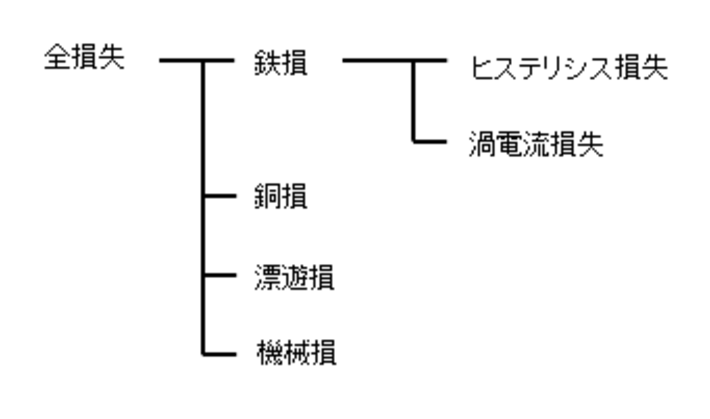
\includegraphics[scale=0.8]{./fig/loss_analysis.pdf}
	\caption{\cite{fdls}}
	\label{fig:loss_analysis}
\end{figure}
\end{enumerate}
\clearpage
\subsection{独自考察}
\begin{enumerate}[1.]
	\item 理想変圧器とは以下の条件を満たす変圧器のことをいう\cite{1130000795154912128}.
\begin{itemize}
	\item 巻線の抵抗が0である.
	\item 鉄心の透磁率が無限大であり,したがって磁気回路における磁気抵抗が0である.
	\item 鉄心の鉄損が0である.
	\item 鉄心の磁気飽和は無視できる.
\end{itemize}
\item 一方,実際の変圧器は理想変圧器と異なり,以下のことを考慮しなければならない
\label{real}
\cite{1130154912128}.
\begin{itemize}
	\item 一次及び二次巻線の抵抗や漏れリアクタンスが存在する.
	\item 主磁束を作るために起磁力,すなわち励磁電流が必要である.
	\item 鉄心中に鉄損が存在する.
	\item 鉄心の磁気飽和を無視することは実際上できないが,ここでは特に考慮しない.
\end{itemize}
\item モータなどにおける損失は大きく分けて,コアに発生する鉄損,コイル巻線(誘導機の場合は二次導体も含む)に発生する銅損,そして,摩擦や空気抵抗に起因する機械損に分類できる.
さらに,負荷によって導体,鉄に生じる損失のうち鉄損,銅損に含まれないものを漂遊負荷損と呼ぶ.
これらをまとめたものを\wfig{loss_analysis}に示す.
\begin{figure}[h]
	\centering
	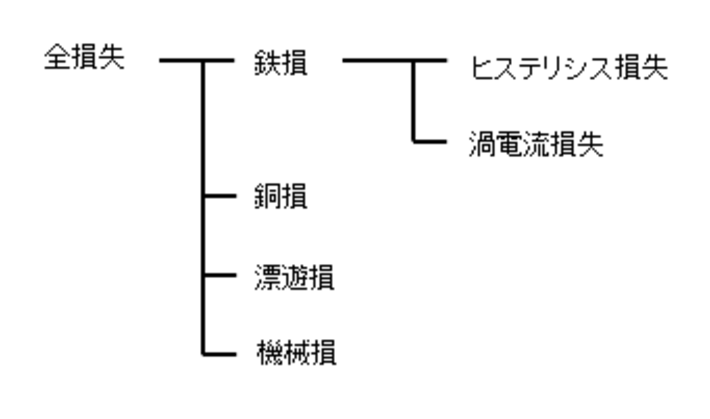
\includegraphics[scale=0.8]{./fig/loss_analysis.pdf}
	\caption{損失の分類\cite{fdls}}
	\label{fig:loss_analysis}
\end{figure}
\end{enumerate}

\clearpage
\section{結論}
本実験を通して以下のことを達成することができた.
\begin{itemize}
	\item 磁気回路と磁性材料についての理解
	\item 変圧器鉄心の交流化特性を測定し,測定原理と鉄心のヒステリシス損算出法の理解
	\item 変圧器における励磁電流,電力,位相差の変化の観測方法の理解
\end{itemize}
\newpage
\printbibliography[title=参考文献]

\end{document}